\documentclass[xcolor={dvipsnames}, 9pt]{beamer}
\usetheme{default}
\usepackage{amsmath, amsfonts, tikz, xcolor, graphicx}
\usepackage[backend=bibtex]{biblatex}
\usepackage[cal = esstix]{mathalpha}
\usefonttheme{serif}

\addbibresource{referensimnb.bib}

\setbeamercolor{background canvas}{bg=BrickRed!25!White}
\renewcommand{\emph}[1]{\textcolor{Blue}{#1}}

%\includeonlyframes{current}

\title{MatNum: Masalah Nilai Batas}
\author{Fadhlannafis K. K., Gema Nadiku Pantouw, Muhammad Ariq Fakhri, Muhammad Arif Wibisono}
\date{10122040, 10122066, 10122076, 10122108}
\begin{document}
	\begin{frame}[plain]
		\maketitle
	\end{frame}
	\begin{frame}{Catatan}
		%PPT ini saya buat untuk menunjang pembelajaran matematika numerik saya, setelah UTS saya di bawah setengahnya rata-rata (alias kuartil 4). \newline
		Pembahasan di PPT ini cenderung teoritik. Kami mengambil referensi dari PPT Bu Lena dan dari:
		\nocite{*}
		\printbibliography
	\end{frame}
	\begin{frame}{Pengantar}
		Suatu \emph{masalah nilai batas} adalah persamaan diferensial (dalam slides ini hanya yang biasa) dengan orde dua atau lebih, sehingga solusi $u$ memenuhi syarat batas
		\begin{align*}
			u(a) = A, u(b) = B.
		\end{align*}
		Sebagai contoh,
		\begin{align*}
			\begin{cases}
				u'' + p(x)u = f(x), & a<x<b, \\
				u(a) = A, u(b) = B.
			\end{cases}
		\end{align*}
		Untuk menyelesaikan masalah nilai batas secara numerik, ada dua metode:
		\begin{enumerate}
			\item Metode Tembakan/\textit{Shooting} Linear,
			\item Metode Beda Hingga.
		\end{enumerate}
	\end{frame}
	\begin{frame}{Metode Tembakan Linear: Pengantar}
        ntar dibenerin \newline
	   Kita tinjau masalah nilai batas linear:
        \begin{gather}
            u''(x) + p(x)u'(x) + q(x)u(x) = r(x), a<x<b, \label{mnb} \\
            u(a) = A, u(b) = B. \nonumber
        \end{gather}
       Asumsikan \eqref{mnb} memiliki solusi tunggal, yaitu $u(x)$. Ide dari metode tebakan linear adalah mendekati masalah \eqref{mnb} dengan suatu masalah nilai awal
       \begin{gather}
           u''(x) + p(x)u'(x) + q(x)u(x) = r(x), a<x<b, \label{mna} \\
            u(a) = A, u'(a) = A' \nonumber
       \end{gather}
       dengan $A'$ dipilih sedemikian sehingga $u(b)=B$. Setelah itu, kita bisa gunakan metode-metode numerik yang biasa digunakan untuk masalah nilai awal.
	\end{frame}
    \begin{frame}{Metode Tembakan Linear: Konstruksi}
        Yang menjadi masalah adalah bagaimana cara memilih $A'$. Kita tebak:
        \begin{align}
        	u'(a) = s_1 \label{tebak1}\\
        	u'(a) = s_2 \label{tebak2}
        \end{align}
        Masalah nilai awal \eqref{mna},\eqref{tebak1} dan \eqref{mna},\eqref{tebak2} dapat diselesaikan. Misalkan solusi dari \eqref{mna},\eqref{tebak1} adalah $v(x)$ dan solusi dari \eqref{mna},\eqref{tebak2} adalah $w(x)$. Kita bisa asumsikan $v(b)\neq B$, $w(b)\neq B$, dan $v\not\equiv w$. Maka $u\not\equiv v$, $u\not\equiv w$. Lalu, karena masalah \eqref{mna} linear, haruslah
        \begin{align*}
        	u(x) = \theta w(x) + (1-\theta)v(x).
        \end{align*}
        untuk suatu $\theta\in\mathbb{R}$. \newline
        Sekarang, agar $u$ menjadi solusi \eqref{mnb}, haruslah
        \begin{align*}
        	\theta w(b) + (1-\theta)v(b) &= B \\
        	\Rightarrow \theta &= \frac{B - v(b)}{w(b)-v(b)}.
        \end{align*}
    \end{frame}
    \begin{frame}{Metode Tembakan Linear: Konstruksi}
    	Dengan \textit{framework} sebelumnya, sekarang kita coba tinjau dua masalah nilai awal berikut:
    	\begin{gather}
    		u''(x) + p(x)u'(x) + q(x)u(x) = r(x), u(a) = A, u'(a) = 0 \label{mna2}\\
    		u''(x) + p(x)u'(x) + q(x)u(x) = 0, u(a) = 0, u'(a) = B \label{mna3}
    	\end{gather}
    	Misalkan solusi dari \eqref{mna2} adalah $v_1$ dan dari \eqref{mna3} adalah $w_1$. Dari kelinearan, kita dapatkan solusi $u$ haruslah memenuhi
    	\begin{align*}
    		u(x) = v_1(x) + \theta w_1(x), \\
    		u(a) = A, u(b) = v_1(b) + \theta w_1(b).
    	\end{align*} 
		Maka
		\begin{align*}
			\theta = \frac{B - v_1(b)}{w_1(b)} \Rightarrow u(x) = v_1(x) + \frac{B - v_1(b)}{w_1(b)}.
		\end{align*}
		Metode ini disebut \emph{metode Shooting/tembakan}, karena seolah-olah kita menembakkan artileri di titik $x=a$ dari ketinggian $A$ sehingga "hadiah" yang kita tembakkan mengenai target di titik $x=b$ dengan ketinggian $B$.
    \end{frame}
    \begin{frame}{Metode Tembakan Linear: Kekonvergenan}
    	Tentunya, kekonvergenan metode tembakan linear sangat bergantung pada metode yang digunakan untuk menyelesaikan masalah nilai awal. Dalam pembahasan ini, kita tinjau masalah nilai batas yang lebih umum:
    	\begin{gather}
    		\vec{y'} = A(x)\vec{y} + \vec{q(x)}, a<x<b \\
    		B_a\vec{y}(a) + B_b\vec{y}(b) = \vec{B} \label{genmnb}
    	\end{gather}
    	dengan mengingat bahwa masalah nilai batas orde-$n$ dapat diubah menjadi sistem persamaan diferensial orde 1. Maka solusi dari \eqref{genmnb} dapat ditulis sebagai
        \begin{align*}
            \vec{y}(x) = Y(x)\vec{s} + \vec{v}(x), a\leq x\leq b
        \end{align*}
        dengan $Y(x)$ adalah suatu solusi fundamental, $\vec{s}$ adalah vektor parameter, dan $\vec{v}(x)$ adalah solusi partikular. Kita asumsikan
        \begin{align*}
            Y'(x) = A(x)Y, a<x<b, Y(a) = I.
        \end{align*}
        Misalkan 
    \end{frame}
    \begin{frame}{Metode Tembakan Linear: Galat}
    	Sekarang akan ditentukan galat dari metode tembakan. Tentunya, seperti konvergensi, galat dari metode ini sangat bergantung pada metode yang digunakan untuk menyelesaikan masalah nilai awal. Tinjau masalah \eqref{genmnb}. \newline
        Misalkan $\tau$ adalah toleransi galat untuk penyelesaian masalah nilai awal. Cara paling mudah untuk meminimalisasi galat adalah dengan mengendalikan galat lokal di $\vec{v}(x)$ dan $Y(x)$ sesuai dengan $\tau$, dan menentukan efeknya pada $\vec{y}(x)$. \newilne
        Asumsikan bahwa setiap solusi numerik dari MNA dicari menggunakan titik-titik
        \begin{align*}
            a = x_1 < x_2 < \cdots < x_N < x_{N+1} = b,
        \end{align*}
        dan setiap solusi numerik $\{\vec{y}_i\}$ memenuhi
        \begin{align*}
            \vec{y}_{i+1} = \Gamma_i\vec{y}_i + \vec{g}_i, i = 1,\dots, N
        \end{align*}
        dengan matriks $\Gamma_i$ dan vektor $\vec{g}_i$ ditentukan dari metode numerik yang digunakan untuk menyelesaikan MNA.
    \end{frame}
    \begin{frame}{Metode Tembakan Linear: Galat}
        
    \end{frame}
    \begin{frame}[fragile]{Metode Tembakan Linear: Kode Matlab}
    	Kode Matlab dari metode tembakan linear bisa ditulis sebagai berikut:
		\begin{verbatim}
			function X = linshoot(a,b,n,p,q,r,xa,xb)
			% Pendefinisian variabel
			h = (b-a)/n;
			X = zeros(n+1,1);
			U = zeros(n+1,1);
			U(1) = xa;
			U1 = zeros(n+1,1);
			U1(1) = 0;
			U2 = zeros(n+1,1);
			V = zeros(n+1,1);
			V(1) = 0;
			V1 = zeros(n+1,1);
			V1(1) = 1;
			V2 = zeros(n+1,1);
		\end{verbatim}
	\end{frame}
	\begin{frame}[fragile]{Metode Tembakan Linear: Kode Matlab}
		\begin{verbatim}
			% Mencari solusi dari u(t)
			U2(1) = p(a)*U1(1) + q(a)*U(1) + r(a);
			for j = 2:1:(n+1)
			U(j) = U(j-1) + h*U1(j-1);
			U1(j) = U1(j-1) + h*U2(j-1);
			U2(j) = p(a+h*(j-1))*U1(1) + q(a+h*(j-1))*U(1) + r(a+h*(j-1));
			end
			% Mencari solusi dari v(t)
			V2(1) = p(a)*V1(1) + q(a)*V(1) + r(a);
			for j = 2:1:(n+1)
			V(j) = V(j-1) + h*V1(j-1);
			V1(j) = V1(j-1) + h*V2(j-1);
			V2(j) = p(a+h*(j-1))*V1(1) + q(a+h*(j-1))*V(1) + r(a+h*(j-1));
			end
			% Mencari solusi dari x(t)
			for j = 1:1:(n+1)
			X(j) = U(j) + ((xb - U(n+1))*V(j))/V(n+1);
			end
			end
		\end{verbatim}
		% JANGAN HAPUS [fragile]
	\end{frame}
    \begin{frame}[fragile]{Metode Tembakan Linear: Contoh}
    	Sebagai contoh, tinjau masalah
    	\begin{align*}
    		x''(t) = tx'(t) - 2x(t) + 2 \\
    		x(a) = 0, x(b) = 1.
    	\end{align*}
    	Di Matlab, tulis
    	\begin{verbatim}
    		a = 0; % Batas bawah t
    		b = 1; % Batas atas t
    		n = 10;% Banyaknya partisi
    		% x(t) = t^2
    		p = @(t) t;
    		q = @(t) -2;
    		r = @(t) 2;
    		xa = 0; % Nilai x(a)
    		xb = 1; % Nilai x(b)
    		X2 = linshoot(a,b,n,p,q,r,xa,xb);
    		T = linspace(a,b,n+1);
    		plot(T,X2)
    		title('Visualisasi Hasil Metode Shooting Linier')
    		xlabel('t')
    		ylabel('x')
    	\end{verbatim}
    \end{frame}
    \begin{frame}{Metode Tembakan Linear: Contoh}
    	Dari kode tersebut, didapat grafik:
    	%\begin{center}
    	%	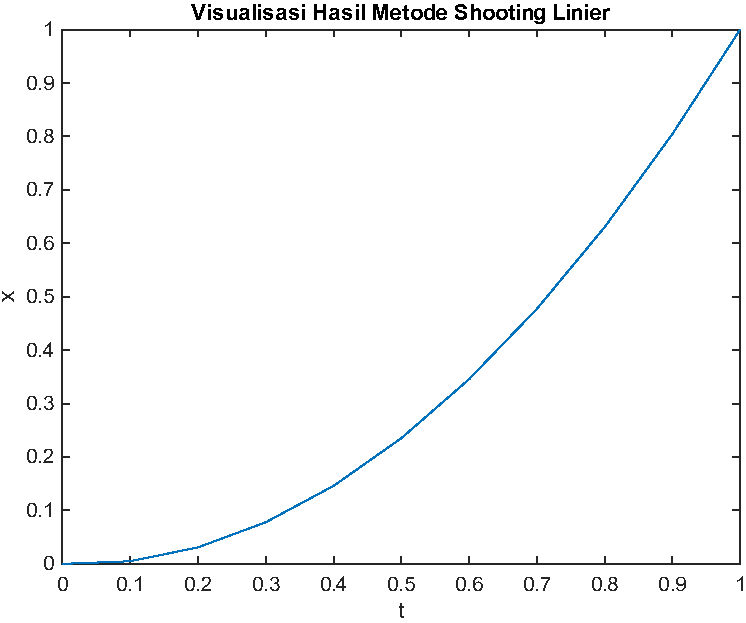
\includegraphics[scale=0.4]{linearshooting.pdf}
    	%\end{center}
    \end{frame}
    \begin{frame}{Metode Beda Hingga: Pengantar}
    	content...
    \end{frame}
%	\begin{frame}{Metode Beda Hingga: Pengantar}
%		kemungkinan salah total, ntar gw bikin t e lax di sini. \newline
%		Pada dasarnya, metode beda hingga ingin mendekati solusi analitik dengan polinom piecewise. Untuk membangun metode beda hingga, di slides ini akan digunakan \emph{prinsip Rayleigh-Ritz} dan \emph{prinsip Galerkin}. Sebelum itu, diperlukan beberapa definisi. \par
%		\begin{definition}[Ruang $L^2$]
%			Misalkan $a,b\in\mathbb{R}, a<b$. \emph{Ruang $L^2(a,b)$} didefinisikan sebagai himpunan semua fungsi $v:[a,b]\to\mathbb{R}$ dengan \emph{hasil kali dalam} yang didefinisikan sebagai
%			\begin{align*}
%				\langle u,v\rangle_{L^2(a,b)} = \left(\int_{a}^{b} |u(x)v(x)| dx\right)^{1/2} < \infty.
%			\end{align*}
%		\end{definition}
%	\end{frame}
%	\begin{frame}{Metode Beda Hingga: Pengantar}
%		\begin{definition}[Ruang Sobolev]
%			Misalkan $k\in\mathbb{N}$, dan $a,b\in\mathbb{R}, a<b$. Kita definisikan \emph{Ruang Sobolev} $H^k(a,b)$ sebagai himpunan semua fungsi $v:[a,b]\to\mathbb{R}$ sehingga $v$ dan turunan-turunannya sampai orde ke $k-1$ kontinu absolut di $[a,b]$ dan $v^{(k)}\in L^2(a,b)$, yang dilengkapi hasil kali dalam
%			\begin{align*}
%				\langle u,v\rangle_{H^k(a,b)} = \left(\sum_{m=0}^{k}\langle u^{(m)},v^{(m)}\rangle_{L^2(a,b)}\right)^{1/2}.
%			\end{align*}
%		\end{definition}
%		\begin{definition}[Ruang Hilbert]
%			Misalkan $(V,\langle\cdot,\cdot\rangle)$ adalah ruang hasil kali dalam terhadap lapangan $\mathbb{F}$. Kita sebut $V$ sebagai \emph{ruang Hilbert} jika terhadap norm $\|v\|=\langle v,v\rangle$, $V$ lengkap, dengan kata lain setiap barisan Cauchy di $V$ konvergen di $V$.
%		\end{definition}
%		\begin{definition}[Ruang Dual]
%			Misalkan $V$ adalah ruang vektor terhadap lapangan $\mathbb{F}$. \emph{Ruang dual} dari $V$, ditulis $V'$, didefinisikan sebagai ruang vektor berisi semua transformasi linear $l:V\to\mathbb{F}$, dengan $l$ disebut \emph{fungsional linear}, dengan operasi jumlah dan perkalian skalar di $\mathbb{F}$.
%		\end{definition}
%	\end{frame}
%	\begin{frame}{Metode Beda Hingga: Konstruksi}
%		Di sini, pertama akan ditinjau konstruksi metode Galerkin pada ruang Hilbert $V$, mengikuti \cite{Han2009Theoretical}. Bisa dibuktikan bahwa ruang $L^2$ dan ruang Sobolev adalah ruang Hilbert. Maka, konstruksi yang ada di sini adalah perumuman dari metode beda hingga. \par
%		Misalkan $V$ adalah ruang Hilbert, $a(\cdot,\cdot):V\times V\to \mathbb{R}$ adalah fungsi yang linear terhadap kedua argumennya (disebut \emph{bilinear}), dan $l\in V'$. Kita akan tinjau masalah
%		\begin{align}\label{fdm_cons1}
%			u\in V, \, a(u,v) = l(v) \, \forall v\in V,
%		\end{align}
%		dengan asumsi $a(\cdot,\cdot)$ terbatas dan $V$-eliptik
%		\begin{align}
%			|a(u,v)|&\leq M\|u\|_V\|v\|_V \, \forall u,v\in V, \label{fdm_cons2} \\
%			a(v,v) &\geq c_0\|v\|_V^2 \, \forall v\in V. \label{fdm_cons3}
%		\end{align}
%		untuk suatu $M,c_0>0$.  
%	\end{frame}
%	\begin{frame}{Metode Beda Hingga: Konstruksi}
%		Teorema berikut menjamin bahwa masalah \eqref{fdm_cons1} memiliki solusi tunggal. 
%		\begin{theorem}[Lemma Lax-Milgram]
%			Misalkan $V$ adalah ruang Hilbert, $a(\cdot,\cdot)$ adalah form bilinear terbatas dan $V$-eliptik di $V$, dan $l\in V'$. Maka ada solusi tunggal dari masalah
%			\begin{align}\label{laxmilgram}
%				u\in V, a(u,v)=l(v) \, \forall v\in V.
%			\end{align}
%		\end{theorem}
%		Bukti. Memerlukan beberapa teorema yang sudah sangat jauh di luar konteks slide ini. Tetapi, idenya adalah menyadari bahwa \eqref{laxmilgram} ekuivalen dengan suatu masalah nilai tetap, lalu gunakan teorema-teorema yang sangat jauh tersebut. $\square$ \newline
%		Tapi, secara umum, sulit menyelesaikan masalah tersebut karena $V$ biasanya berdimensi tak hingga.
%	\end{frame}
%	\begin{frame}{Metode Beda Hingga: Konstruksi}
%		Dengan asumsi \eqref{fdm_cons2}, \eqref{fdm_cons3}, kita batasi masalah \eqref{fdm_cons1} ke subruang $V_n\subset V$ yang berdimensi $n$, yaitu
%		\begin{align}\label{fdm_cons4}
%			u_n\in V_n, \, a(u_n, v) = l(v), \, \forall v\in V_n.
%		\end{align}
%		Karena $V_n$ berdimensi hingga, kita bisa definisikan basis $\{\phi_i\}_{i=1}^n$ sehingga
%		\begin{align*}
%			u_n = \sum_{j=1}^{n} \xi_j\phi_j.
%		\end{align*}
%		Sekarang dengan menuliskan $v$ sebagai $\phi_i$ di \eqref{fdm_cons4} untuk setiap $i$, kita dapatkan SPL
%		\begin{align}
%			A\vec{\xi} = \vec{b}
%		\end{align}
%		dengan $A = [a(\phi_j,\phi_i)]$, $\vec{\xi} = [\xi_j]$, dan $\vec{b} = [l(\phi_i)]$. Maka \eqref{fdm_cons4} bisa diselesaikan dengan cara menyelesaikan SPL seperti di ALE.
%	\end{frame}
%	\begin{frame}{Metode Beda Hingga: Konstruksi}
%		Tentunya solusi $u_n$ secara umum akan berbeda dari $u$. Agar solusi lebih akurat, bisa ditentukan solusi $u_N$ di $V_N\subset V$ sehingga $N>n$. Maka, untuk suatu barisan subruang $V_{n_1} \subset V_{n_2} \subset \cdots \subset V$, kita bisa hitung suatu barisan solusi $u_{n_i}\in V_{n_i}$. Prosedur ini disebut \emph{metode Galerkin}. \newline
%		Sekarang kita akan tinjau masalah \eqref{fdm_cons1} di ruang Sobolev. Sebelum itu, perlu dikenalkan
%        \begin{definition}
%            \begin{enumerate}
%                \item Misalkan $A,B\in\mathbb{R}$. Kita definisikan $H^1_E(a,b)$ sebagai himpunan semua fungsi $v\in H^1(a,b)$ sehingga $v(a)=A, v(b)=B$.
%                \item Kita definisikan $H^1_0(a,b)$ sebagai himpunan semua fungsi $v\in H^1(a,b)$ sehingga $v(a)=v(b)=0$.
%            \end{enumerate}
%        \end{definition}
%	\end{frame}
%    \begin{frame}{Metode Beda Hingga: Konstruksi}
%        Kita tinjau masalah nilai batas
%        \begin{gather}
%            -\frac{d}{dx}\left(p(x)\frac{du}{dx}\right) + q(x)\frac{du}{dx} + r(x)u = f(x), a<x<b, \label{mnb3} \\
%            u(a) = A, u(b) = B \nonumber \\
%            p\in C^1[a,b], r\in C[a,b], f\in L^2[a,b], p(x)\geq c_0>0, r(x)\geq 0. \nonumber
%        \end{gather}
%        Untuk menyelesaikan masalah tersebut, kita definisikan
%        \begin{align}\label{weakform}
%            \mathcal{I}(u) = \frac{1}{2}\int_a^b (p(x)(u')^2+r(x)u^2) dx - \int_a^b f(x)u(x)dx
%        \end{align}
%        dengan $u\in H^1_E(a,b)$, dan kita tinjau masalah optimisasi
%        \begin{align}\label{rayleighritz}
%            \min_{u\in H^1_E(a,b)} \mathcal{I}(u).
%        \end{align}
%        yang disebut sebagai \emph{prinsip Rayleigh-Ritz}. Nanti akan dibuktikan bahwa fungsi yang menjadi solusi masalah tersebut juga menyelesaikan masalah nilai batas di awal.
%    \end{frame}
%    \begin{frame}{Metode Beda Hingga: Konstruksi}
%       Definisikan suatu form bilinear simetrik di $H^1(a,b)$:
%       \begin{align*}
%           \mathcal{A}(w,v) = \int_a^b (p(x)w'(x)v'(x)+r(x)w(x)v(x)) dx.
%       \end{align*}
%       Akibatnya, kita bisa tulis \eqref{weakform} sebagai
%       \begin{align}\label{weakform2}
%           \mathcal{I}(w) = \frac{1}{2}\mathcal{A}(w,w) - \langle f,w\rangle_{L^2(a,b)}, \, w\in H^1_E(a,b).
%       \end{align}
%       Dengan formulasi seperti ini, kita punya teorema.
%       \begin{theorem}[Ekuivalensi Prinsip Rayleigh-Ritz]
%           Suatu fungsi $u\in H^1_E(a,b)$ meminimumkan $\mathcal{I}$ di $H^1_E(a,b)$ jika dan hanya jika $u$ memenuhi \emph{prinsip Galerkin}
%           \begin{align}\label{galerkin}
%               \mathcal{A}(u,v) = \langle f,v\rangle_{L^2(a,b)} \, \forall v\in H^1_0(a,b).
%           \end{align}
%       \end{theorem}
%       Bukti. Dijamin dari Lemma Lax-Milgram. $\square$ \newline
%       Tentunya mencari solusi untuk masalah \eqref{weakform} juga sulit. Maka, kita bisa gunakan metode Galerkin yang sudah didefinisikan sebelumnya.
%    \end{frame}
%    \begin{frame}{Metode Beda Hingga: Konstruksi}
%        Kita batasi masalah nilai batas \eqref{mnb} pada subruang berdimensi-$n>2$ $S_E^n\subset H_E^1(a,b)$. Salah satu cara paling mudah adalah dengan mendefinisikan fungsi $\psi\in H_E^1(a,b)$, misalkan
%		\begin{align*}
%			\psi(x) = \frac{B-A}{b-a}(x-a)+A
%		\end{align*}
%		dan fungsi-fungsi $\phi_j\in H_0^1(a,b), j = 1,\dots,n-1$ yang bebas linear, dan mendefinisikan
%		\begin{align*}
%			S_E^n = \{v_n\in H_E^1(a,b) : v_n = \psi + \sum_{i=1}^{n-1}a_i\phi_i, a_i\in\mathbb{R}\}.
%		\end{align*}
%		Kita tinjau suatu aproksimasi dari masalah Rayleigh-Ritz:
%		\begin{align*}
%			\min_{w_n \in S_E^n} \mathcal{I}(w_n),
%		\end{align*}
%		dan tentunya kita punya teorema yang merupakan aproksimasi dari Prinsip Galerkin. Hal tersebut kita sebut sebagai \emph{metode Galerkin}.
%    \end{frame}
%    \begin{frame}{Metode Beda Hingga: Konstruksi}
%    	Sekarang dari metode Galerkin, akan dikonstruksi metode beda hingga. 
%    \end{frame}
\end{document}
